
\documentclass[twocolumn, amsmath]{revtex4}

\usepackage{graphicx}
%\graphicspath{ {tex_pics/} }


\begin{document}


\title{PHYS 605 Lab \#6} 

\author{Morgan A. Daly}
\author{Evin O'Shea}
\date{\today} 


\maketitle


\section{Introduction and Theory}
\subsection{Purpose}

In this lab, the focus was to learn about how diodes can be used in AC circuits. The first part of the lab showed how a single diode can be used as a half-wave rectifier. In the second part of the lab the group made a full wave rectifier. In the third part of the lab the behavior of a zener diode was explored both with DC and AC voltage sources.

\subsection{Background / Theory}

The lab revolved around the behavior of diodes in AC circuits. Diodes are an interesting type of passive circuit element which have interesting properties. The most important property of diodes is that they only allow current flow in one direction. When an AC voltage source powers a diode, only the positive or negative voltage will go through the diode. 
%not sure where to put this if at all
%The second interesting property of diodes is that they have a minimum voltage required to pass current through/ has a max? clipps the voltage?

In the Part A of the lab a diode was used to convert the AC signal into only a positive signal. This demonstrated the diode property of only allowing current flow in one direction. When the AC source supplies a positive voltage the diode would allow current flow through. When the voltage source supplies a negative voltage the diode will not let current flow through. The circuit used for this part of the lab was built in two aprts. First the circuit was built with a resistor and a diode in series with the oscilliscope connected in parallel with the voltage source and the diode. After this circuit was investigated a 3V DC supply was added to the circuit between the resistor and diode. The final circuit for this part of the lab is shown below:

\begin{figure}
    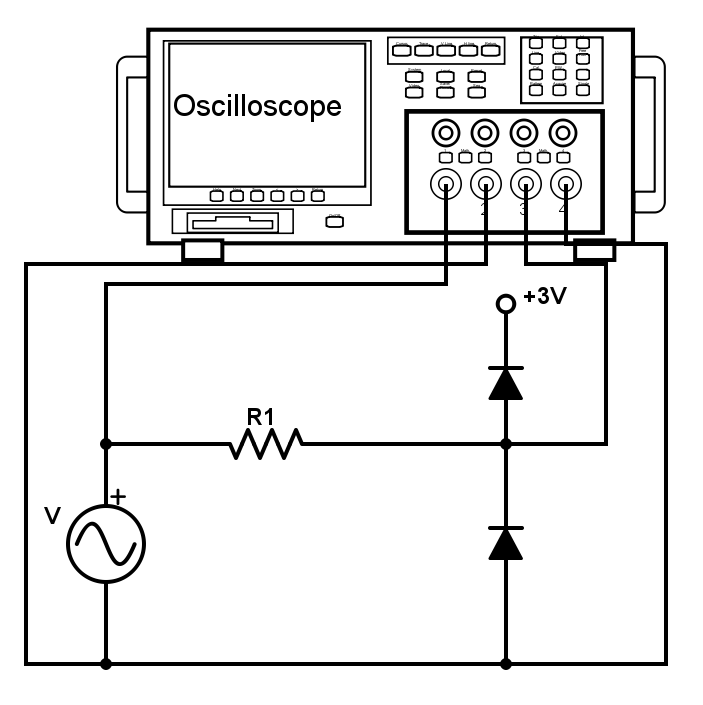
\includegraphics[scale=0.3]{halfwave.png}  
    \caption{This circuit only supplies postive voltage to the oscilloscope.}
\end{figure}

In the second part of the lab, the diode was used to allow the positive and negative voltages through while inverting the negative voltage. The circuit used for this part of the lab is shown below:

\begin{figure}
    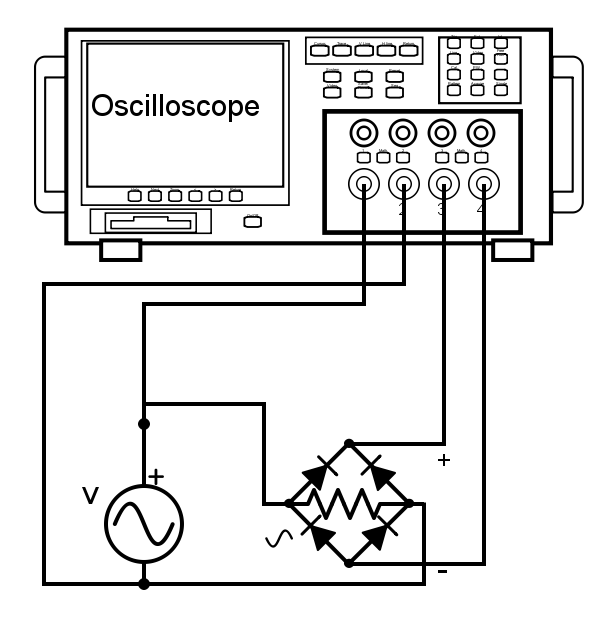
\includegraphics[scale=0.3]{bridge.png}  
    \caption{A full wave rectifier with input and output connected to an ocsilloscope}
\end{figure}

The circuit makes all the voltage positive. As positive voltage is supplied to the circuit current will pass through the top left diode and not the bottom left because of the orientation of the diode. Current will then flow down through the resistor and not the top right diode. As negative voltage is supplied to the circuit current will flow from the bottom side of the AC source. As the current flows to the right side of the bridge it will pass through the top right diode and not the bottom right. The current will then flow down through the resistor as it did when a positive voltage was supplied. This combination will cause flow in only one direction through the resistor and the output of the bridge.

For the third part of the lab, a zener diode was investigated. The distinction between a regular diode and a zener diode is that a zener diode will allow voltage to pass in both directions, but in the reverse-bias direction, there is a minimum voltage required to cause current flow. This voltage is called the zener voltage. A diagram of the circuit for this part of the lab is shown below:

\begin{figure}
    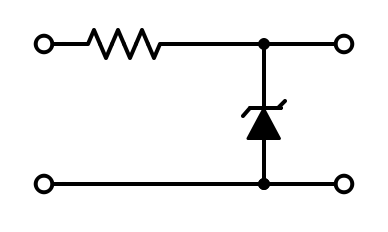
\includegraphics[scale=0.3]{zener.png}  
    \caption{This circuit only supplies postive voltage to the oscilloscope.}
\end{figure}

The left side was connected to both DC and AC sources to invesitage different properties of the zener diode. 
%One important use of the zener diode was to "clip" the voltage source. This means that the zener diode caps the voltage allowed through... 
%********need to add more when I can see plots******





\section{Methodology}

\begin{enumerate}
    \item Construct RC circuit with oscilloscope as show in figure (1) without the 3V DC source and diode attatched.
    \item Take record of the plot from the oscilloscpe.
    \item Adjust frequency and amplitude of input source and repeat step 2.
    \item Build diode brdge shown in figure (2).
    \item Connect input source (one that is external from the protoboard) and connect the oscilloscope as shown in figure (2).
    \item Repeat steps 2 and 3 to get data about the bridge.
    \item Construct the circuit shown in figure (3).
    \item Add an adjustable DC input to the left side of the circuit and connect a measurement device to the right side of the circuit.
    \item Make recordings of the output voltages as the input voltage is modified.
    \item Swap the DC input for an AC input and swap the measurement device for one suited for AC voltages (oscilloscope) if necessary.
    \item Take record of the plot shown on the oscilloscope.
    \item Swap the zener diode out for another one and repeat step 11.
    \item Combine the two diodes in series in the same direction and make record of the plot on the oscilloscope.
    \item Combine the two zener diodes in parallel in opposite directions to "clip" both positive and negative voltages from the AC input.
\end{enumerate}


\section{Results and Analysis}

\subsection{Data}
For part A of the lab, first only part of the circuit was built as described previously. This setup was investigated with varying voltages and frequencies for the input source.


The input source was initially set to an amplitude and frequency of 2.64V and 7.225Hz respectively. The $V_{max}$ for the diode was 1.80V.

\begin{figure}
    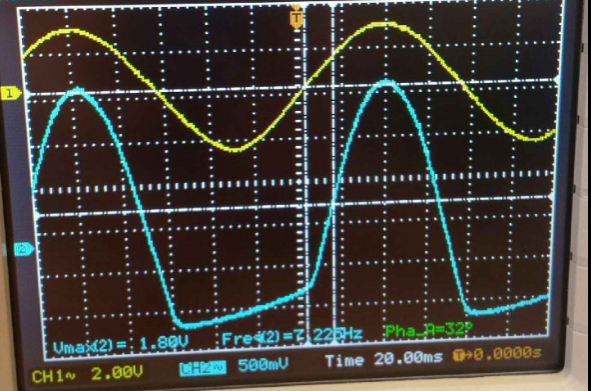
\includegraphics[scale=0.3]{1800mV.png}  
    \caption{This circuit only supplies postive voltage to the oscilloscope.}
\end{figure}


second amplitude: 4.08V f=7.225Hz
-V2(max) 2.72V

\begin{figure}
    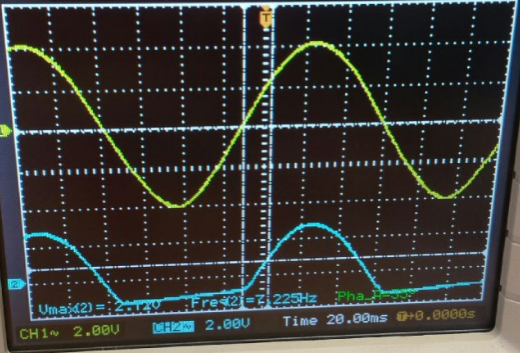
\includegraphics[scale=0.3]{2720mV.png}  
    \caption{This circuit only supplies postive voltage to the oscilloscope.}
\end{figure}


third frequency: 2.64V f=75.19Hz
-V2(max) 1.76V

\begin{figure}
    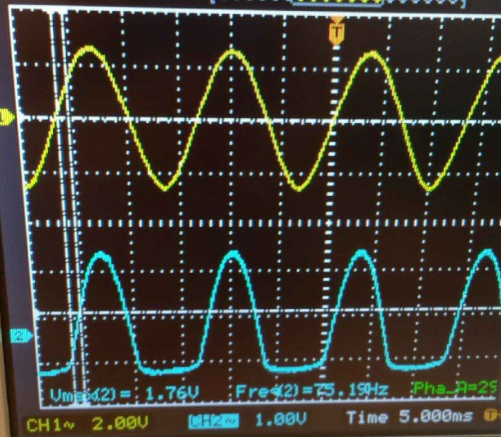
\includegraphics[scale=0.3]{1760mV.png}  
    \caption{This circuit only supplies postive voltage to the oscilloscope.}
\end{figure}

%fourth frequency: same for higher

After adjusting the amplitude and frequency of the input voltage a 3.065V DC source was added to the circuit attatched by another diode as shown in figure (1). 

The input voltage and frequency were first set to 2.64V and 731.0mHz respectively. The $V_{max}$ for the diode was 464mV.
V2 464mV

\begin{figure}
    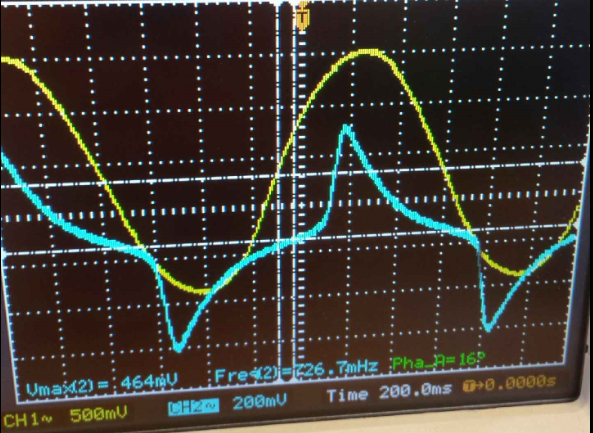
\includegraphics[scale=0.3]{464mV.png}  
    \caption{This circuit only supplies postive voltage to the oscilloscope.}
\end{figure}



second: 2.64V  74.63Hz
V2 480mV

\begin{figure}
    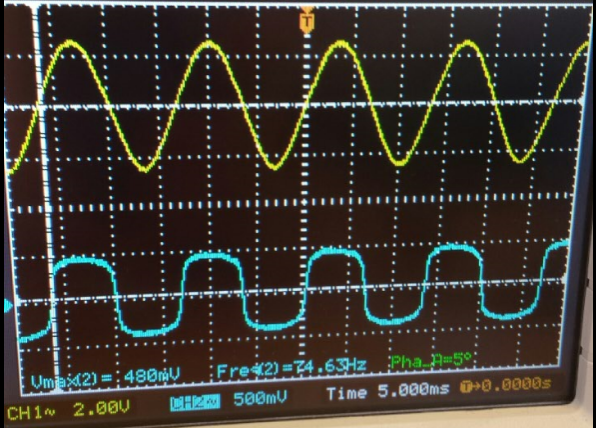
\includegraphics[scale=0.3]{480mV.png}  
    \caption{This circuit only supplies postive voltage to the oscilloscope.}
\end{figure}

third: 1.48V f=7.225
v2 460mV

\begin{figure}
    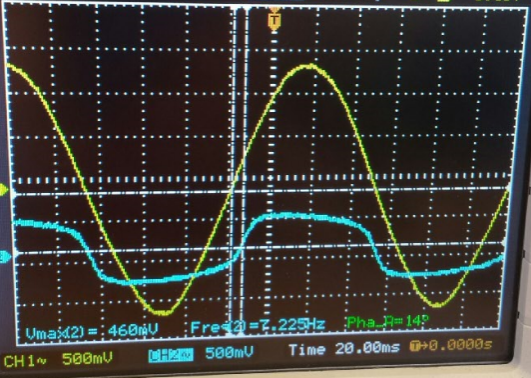
\includegraphics[scale=0.3]{460mV.png}  
    \caption{This circuit only supplies postive voltage to the oscilloscope.}
\end{figure}




%\subsection{Calculations}



 
\subsection{Analysis}


\section{Conclusion}
The relationship between frequency, impedance, and voltage was made obvious, and observations matched expectations based on known equations. The resulting improved understanding and intuition for a new type of circuit makes this successful.

Measured values of gain were compared to calculated values with some error, which seemed to increase at extreme values. The roll off was calculated, and the group was able to observe the behavior of a RC circuit in frequencies that were a part of the filtered frequencies.

\end{document}

